\section{ORB raksturpunktu pāru noteikšanas algoritms}\label{sec:orb}
Iepriekšējās nodaļās attēlu raksturpunktu detektēšana (FAST) un
deskriptoru noteikšana (BRIEF) tika apskatītas atsevišķi. Lai arī tie
algoritmi ir neatkarīgi, tos
var izmantot kā komponentes augstākas abstrakcijas algoritmos, kāds ir ORB,
līdzīgi kā zemākas abstrakcijas algoritmi ir
definēti ar matemātiskām operācijām, transformācijām vai citiem algoritmiem.

ORB izmanto FAST-9 par raksturpunktu noteikšanas komponenti
 un rBRIEF 
(rotācijas invariantu BRIEF modifikāciju) par raksturpunktu salāgošanas
komponenti~\cite{ORB}.
\begin{figure}[tbh]
	\centering
	\def\svgwidth{\linewidth}
	{\small\section{ORB raksturpunktu pāru noteikšanas algoritms}\label{sec:orb}
Iepriekšējās nodaļās attēlu raksturpunktu detektēšana (FAST) un
deskriptoru noteikšana (BRIEF) tika apskatītas atsevišķi. Lai arī tie
algoritmi ir neatkarīgi, tos
var izmantot kā komponentes augstākas abstrakcijas algoritmos, kāds ir ORB,
līdzīgi kā zemākas abstrakcijas algoritmi ir
definēti ar matemātiskām operācijām, transformācijām vai citiem algoritmiem.

ORB izmanto FAST-9 par raksturpunktu noteikšanas komponenti
 un rBRIEF 
(rotācijas invariantu BRIEF modifikāciju) par raksturpunktu salāgošanas
komponenti~\cite{ORB}.
\begin{figure}[tbh]
	\centering
	\def\svgwidth{\linewidth}
	{\small\section{ORB raksturpunktu pāru noteikšanas algoritms}\label{sec:orb}
Iepriekšējās nodaļās attēlu raksturpunktu detektēšana (FAST) un
deskriptoru noteikšana (BRIEF) tika apskatītas atsevišķi. Lai arī tie
algoritmi ir neatkarīgi, tos
var izmantot kā komponentes augstākas abstrakcijas algoritmos, kāds ir ORB,
līdzīgi kā zemākas abstrakcijas algoritmi ir
definēti ar matemātiskām operācijām, transformācijām vai citiem algoritmiem.

ORB izmanto FAST-9 par raksturpunktu noteikšanas komponenti
 un rBRIEF 
(rotācijas invariantu BRIEF modifikāciju) par raksturpunktu salāgošanas
komponenti~\cite{ORB}.
\begin{figure}[tbh]
	\centering
	\def\svgwidth{\linewidth}
	{\small\section{ORB raksturpunktu pāru noteikšanas algoritms}\label{sec:orb}
Iepriekšējās nodaļās attēlu raksturpunktu detektēšana (FAST) un
deskriptoru noteikšana (BRIEF) tika apskatītas atsevišķi. Lai arī tie
algoritmi ir neatkarīgi, tos
var izmantot kā komponentes augstākas abstrakcijas algoritmos, kāds ir ORB,
līdzīgi kā zemākas abstrakcijas algoritmi ir
definēti ar matemātiskām operācijām, transformācijām vai citiem algoritmiem.

ORB izmanto FAST-9 par raksturpunktu noteikšanas komponenti
 un rBRIEF 
(rotācijas invariantu BRIEF modifikāciju) par raksturpunktu salāgošanas
komponenti~\cite{ORB}.
\begin{figure}[tbh]
	\centering
	\def\svgwidth{\linewidth}
	{\small\input{img/orb.pdf_tex}}
	\caption{ORB algoritma blokshēma.}
	\label{fig:orb-sheem}
\end{figure}
Papildus lokālo maksimumu atlasei, ko veic FAST algoritms, ORB izmanto
Harisa (\termEn{Harris}) stūra mēru, lai no FAST raksturpunktiem atlasītu
$N$ skaitu labākos elementus~\cite{ORB}.
Rublē~u.c.\cite{ORB} to pamato ar relatīvi lielo FAST jutību attēla
objektu malām (pretstatā stūriem). Vienkāršota algoritma blokshēma attēlota
\ref{fig:orb-sheem}~attēlā.

FAST definīcija apskatīta \ref{sec:fast}~nodaļā
(\pageref{sec:fast}~lapā) un BRIEF definīcija --- \ref{sec:brief}~nodaļā
(\pageref{sec:brief}~lapā). Pārējās ORB algoritma komponenšu definīcijas
tiks apskatītas turpmākajās apakšnodaļās.

\subsection{Komponentes}
\input{orb.harris.tex}
\input{orb.ofast.tex}
\input{orb.rbrief.tex}


%~ \input{orb.opencv.tex}

%~ \subsection{Potenciālās ātrdarbības uzlabojumu analīze}
%~ \TODO


}
	\caption{ORB algoritma blokshēma.}
	\label{fig:orb-sheem}
\end{figure}
Papildus lokālo maksimumu atlasei, ko veic FAST algoritms, ORB izmanto
Harisa (\termEn{Harris}) stūra mēru, lai no FAST raksturpunktiem atlasītu
$N$ skaitu labākos elementus~\cite{ORB}.
Rublē~u.c.\cite{ORB} to pamato ar relatīvi lielo FAST jutību attēla
objektu malām (pretstatā stūriem). Vienkāršota algoritma blokshēma attēlota
\ref{fig:orb-sheem}~attēlā.

FAST definīcija apskatīta \ref{sec:fast}~nodaļā
(\pageref{sec:fast}~lapā) un BRIEF definīcija --- \ref{sec:brief}~nodaļā
(\pageref{sec:brief}~lapā). Pārējās ORB algoritma komponenšu definīcijas
tiks apskatītas turpmākajās apakšnodaļās.

\subsection{Komponentes}
\subsubsection{Raksturpunktu atlase pēc Harisa mēra}
ORB izmanto FAST9 algoritma noteikto raksturpunktu pēcapstrādi novērtējot tos
pēc Harisa (\termEn{Harris}) stūru mēra un atlasot $N$ skaitu
raksturpunktus ar augstākajiem Harisa mēra rādītājiem~\cite{ORB}.
FAST detektora slieksnis $t$ tiek izvēlēts pietiekami zems, lai
raksturpunktu kopā būtu vismaz $N$ skaits elementu un $t$ tiek samazināts,
ja tā nav~\cite{ORB}.
Šī ir otrreizēja raksturpunktu atlase, jo tiek veikta pēc FAST 
lokālo maksimumu atlases.

%~ Harisa stūra mērs balstās uz starpību kvadrātu summu starp attēla
%~ apgabalu un no tā nobīdītiem apgabaliem, kura aprēķināšanai
%~ Haris\cite{Harris} definē aproksimācijas tenzoru~\cite{FAST}:
%~ \[
	%~ \vb{H} =
	%~ \begin{pmatrix}
		%~ \overline{{I_x'}^2} & \overline{{I_x'}{I_y'}}\\
		%~ \overline{{I_x'}{I_y'}} & \overline{{I_y'}^2}
	%~ \end{pmatrix}
%~ \]
%~ kur $I_x'$ un $I_y'$ ir attēla parciālie atvasinājumi (pēc $x$ un $y$),\\
%~ un
Harisa stūru mērs tiek izmantots Harisa stūru detektorā~\cite{Harris}\cite{FAST},
kuru aprēķina ar:
\begin{equation}
	V_H = |\vb{H}| - k \cdot {(H_{11}+H_{22})}^2
\end{equation}
kur\\
$\vb{H}$ ir Harisa matrica\cite{Harris}\cite{FAST}, un\\
%$H_{11}$ un $H_{22}$ ir $\vb{H}$ matricas elementi, un\\
$k$ ir konstante, kas kontrolē stūra vai malas jutību.

Harisa matrica $\vb{H}$, saīsinātā formā un izvērstā formā,
tiek pierakstīta kā~\cite{Harris}\cite{FAST}:
\begin{equation}\label{eq:harris}
	\vb{H} =
		\begin{pmatrix}
			\langle I_x^2 \rangle & \langle I_xI_y \rangle \\
			\langle I_xI_y \rangle & \langle I_y^2 \rangle
		\end{pmatrix}
		=
		\sum_{\vec{r}} W(\vec{r})
			\begin{pmatrix}
				I_x(\vec{p}+\vec{r})^2 & I_x(\vec{p}+\vec{r}) I_y(\vec{p}+\vec{r}) \\
				I_x(\vec{p}+\vec{r}) I_y(\vec{p}+\vec{r}) & I_y(\vec{p}+\vec{r})^2
			\end{pmatrix}
\end{equation}
kur\\
$I_x$ un $I_y$ ir parciālie atvasinājumi attēlam $\vb{I}$,\\
stūra iekavas $\langle {\,} \rangle$ apzīmē summēšanu noteiktā logā
(saīsinātā forma),\\
$W$ ir izvēlētais logs (kā funkcija), un\\
$\vec{r}$ ir loga pārvietojums no centra punkta $\vec{p}$, kurā tiek noteikta
intensitāšu starpība (atvasinājums).

%~ Harisa stūra detektors balstās uz noteikta attēla loga un tā pārvietojumu
%~ pašlīdzības noteikšanu ar starpību kvadrātu summu, ko
%~ aproksimē \eqref{eq:harris} definīcija~\cite{Harris}.

Hariss~un~Stefens\cite{Harris} (\termEn{Harris~and~Stephen})
rekomendē izmantot Gausa matricu par logu
$W$, bet avots~\cite{ORB}, definējot ORB, izmantotos parametrus nenorāda.
Autors analizējot ORB OpenCV implementācijas pirmkodu\cite{OpenCV-src}
secina, ka ORB implementācijā tiek izmantots $7 \times 7$ kvadrāta formas
logs (ar vienmērīgu sadalījumu) un izmantotais $k=0.04$.

Ņemot vērā, ka Harisa stūru mērs $V_H$ tiek noteikts punktiem
$\vec{p} \in \hat{F_9}(\vb{I}, \vec{p}, t)$, kas ir apakškopa no attēla
$\vb{I}$, pretstatā Harisa stūru detektoram, kas $V_H$ nosaka visiem attēla
punktiem~\cite{Harris}, var arī uzskatīt, ka šajā gadījumā FAST funkcionē kā
filtrs Harisa stūru detektoram.

\subsubsection{oFAST: raksturpunkta virziens} \label{sec:ofast}
oFAST ir ORB algoritma raksturpunktu virziena noteikšanas metode.
Neskatoties uz Rublē~u.c.\cite{ORB} piedēvēto nosaukumu, oFAST tiešā veidā
nemodificē FAST algoritmu un tādēļ autors to uzskata par atsevišķu ORB
algoritma komponenti.

Raksturpunktu virziena informācija ir nepieciešama
ORB rotācijas invariances nodrošināšanai~\cite{ORB}
(sk.~\ref{sec:rbrief-def}~nod.).
Tā noteikšanai izmanto
,,intensitātes centroīdu''\cite{Rosin}\cite{ORB} (jeb ,,masas'' centru, pēc fizikālās
līdzības), kas ir definēta kā:
\begin{equation}
	\vec{C} = \left( \frac{m_{10}}{m_{00}},\; \frac{m_{01}}{m_{00}} \right)
\end{equation}
kur $m_{00}$, $m_{01}$, $m_{10}$ ir attēla momenti, kurus aprēķina pēc:
\begin{equation}
	m_{pq} = \sum_{x,y} x^p y^p I(x,y)
\end{equation}

oFAST virzienu uzdod kā leņķi, kas vienāds ar centroīdas $\vec{C}$
lenķi pret $x$ asi (tās pozitīvo virzienu), ko aprēķina ar~\cite{ORB}:
\begin{equation}
	\theta = \mathrm{atan2}(m_{01}, m_{10})
\end{equation}
kur $\mathrm{atan2}()$ ir divu argumentu arktangenss (kas arī nosaka kvadrantu).

Lai šo virziena mēru padarītu maksimāli rotācijas invariantu,
momentu noteikšanai izvēlas riņķa formas attēla apgabalu ar diametru, kas
vienāds ar salāgotāja (kvadrāta formas) apgabala malas garumu $S$
(definēta~\ref{sec:brief}~nodaļā).

\subsubsection{rBRIEF deskriptors} \label{sec:rbrief-def}
rBRIEF ir rotācijas invarianta modifikācija
BRIEF deskriptoram (sk.~\ref{sec:brief}~nod.),
kura tiek izmantota par salāgošanas komponenti ORB
algoritmam. Idejas pamatā ir aprēķināt BRIEF deskriptoru izmantojot
rotētas salīdzināšanas pāru punktu koordinātes, rotācijas leņķi nosakot pēc
raksturpunkta virziena komponentes (sk.~\ref{sec:ofast}~nod.).

Apzīmēsim rBRIEF deskriptoru ar $D_{n_d}$, kuru mēs varam definēt
pievienojot BRIEF deskriptoram $B_{n_d}$ rotācijas komponenti ar leņķi $\theta$:
\begin{equation}\label{eq:rbrief}
	D_{n_d}(\hat{\vb{p}}, \theta) := \sum_{i=1}^{n_d} 2^{i-1}
		\tau\left(\hat{\vb{p}},
		          \vb{R}(\theta) \times \vb{a}_i,
		          \vb{R}(\theta) \times \vb{b}_i\right)
\end{equation}
kur $\vb{R}(\theta)$ ir rotācijas matrica leņķim $\theta$, kas ir definēta kā:
\[
	\vb{R}(\theta) = 
		\begin{pmatrix}
			\cos\theta & -\sin\theta\\
			\sin\theta & \cos\theta
		\end{pmatrix}
\]

Uzdotā definīcija \eqref{eq:rbrief} ir idejiski ekvivalenta bet 
pierakstīta ievērojami citādāk nekā \cite{ORB} avotā, jo 
Rublē~u.c. visai liberāli reinterpretē mainīgo nozīmi.

Jānorāda, ka nodrošinot rotācijas invarianci, šī informācija tiek
,,atmesta'' no deskriptora, kas samazina tā varianci un tādējādi arī
tā diskriminitāti. Rublē~u.c.\cite{ORB}, šī samazinājuma kompensēšanai,
izstrādā mašīnmācīšanās metodes, ar kuru palīdzību tiek izvēlēti
salīdzināšanas pāri ar augstāko varianci. Izvēlētie punkti attēloti
\ref{fig:pattern2}a.~attēlā un ir novērojama salīdzināšanu pāru tendence
orientēties raksturpunkta rotācijas virzienā (attēlā virzienā uz augšu).
\begin{figure}[tbh]
	\centering
	\def\svgwidth{0.7\linewidth}
	{\input{img/rBRIEF.pdf_tex}}
	\caption{Mašīnmācīšanās metožu izvēlēti salīdzināšanas pāri
		(attēloti 64 pāri)~\cite{ORB}.}
	\label{fig:pattern2}
\end{figure}
Bet ir arī novērojams, ka izvēlētie pāri ir izvietoti līdzīgi, kas palielina
to savstarpējo korelāciju
un tādējādi samazina to informatīvo vērtību. Rublē~u.c.\cite{ORB} izvēles
kritēriju papildina atlasot augstākās variances pārus, kuri atbilst
noteiktam korelācijas slieksnim (sk.~\ref{fig:pattern2}b.~att.), panākot
augstāku kopējo deskriptora diskriminitāti.



%~ \subsection{OpenCV ORB implementācija}
%~ \subsubsection{OpenCV ORB implementācija}
OpenCV biblotēka\cite{OpenCV-src} piedāvā ORB algoritma implementāciju.
Šī implementācija ir pielāgota secīgai izpildei CPU platformai,
bet tā ir pilnībā skalāra un nesatur būtiskus platformas specifiskus
ātrdarbības uzlabojumus (neskaitot \ref{sec:fast-ocv}~nod.~apskatīto
OpenCV FAST implementāciju, kas izmanto SSE2 SIMD instrukcijas).
rBRIEF salīdzināšanas pāri ir kodā definētas konstantes un
OpenCV nesatur ne saskarnes atbalstu, ne rīkus jaunas salīdzināšanas pāru 
kopas ģenerēšanai ar \ref{sec:rbrief-def}~nodaļā aprakstīto mašīnmācīšanās
metodi.

Rublē~u.c.\cite{ORB}, izstrādājot ORB, diskretizē virziena leņķi $\theta$ ar soli
$\frac{2\pi}{30}$ un aprēķina rBRIEF salīdzināšanas pāru koordinātas katrai no
$\theta$ ieņemamajām vērtībām, izveidojot apjomīgu
,,uzmeklēšanas datubāzi'' (\termEn{look-up table}).
OpenCV šo risinājumu nerealizē, tā vietā --- katra raksturpunkta
deskriptora
salīdzināšanas pāru punktu koordinātas tiek pārrēķinātas 
izmantojot rotācijas matricu kā definēts \eqref{eq:rbrief}~\cite{OpenCV-src}.

OpenCV ORB implementācija testos uzrādīja reāla laika spējīgu
apstrādes ātrumu --- virs 30 kadriem sekundē --- trim no četrām testētajām
ierīcēm (sk.~pielikumu~\ref{appx:test4}).
Salīdzinājums ar GPU implementāciju seko nākamajā (\ref{sec:orb-ocv-cl})
apakšnodaļā.

%~ \subsubsection{OpenCV ORB implementācijas OpenCL versija}
\subsubsection{OpenCL versija}
\label{sec:orb-ocv-cl}
OpenCV bibliotēka piedāvā arī OpenCL ORB versiju izpildei
GPU~\cite{OpenCV-src}. GPU implementācijas galvenā atšķirība no CPU versijas 
ir izpildes pavedienu izveide elementu apstrādei, bet, citādi,
algoritma implementācijas uzbūve ir identiska ar CPU implementāciju.
ORB algoritma OpenCL versijas izpildi var izdalīt vairākos etapos, kuri
uzskaitīti \ref{tbl:orb-ocl-steps}~tabulā.
\begin{table}[thb]\small
	\centering
	\caption{ORB GPU implementācijas izpildes etapi.}
	\label{tbl:orb-ocl-steps}
	\vspace{4pt}
	\begin{tabular}{clcl}
		\toprule
		\textbf{Nr.} & \textbf{Darbība} & $N_e$ & \textbf{Pavediena apstrādājamā vienība}\\
		\midrule
		1. & Attēlu piramīdas izveide & $N_L$ & Rezultējošā attēla pikselis\\
		2. & FAST9 punktu klasifikācija & $N_L$ & Attēla pikselis\\
		3. & FAST9 lokālo maksimumu atlase & $N_L$ & Raksturpunkts\\
		4. & Atlase pēc Harisa stūra mēra & 1 & Raksturpunkts\\
		5. & Intensitāšu centroīdu noteikšana & 1 & Raksturpunkts\\
		6. & Attēlu Gausa filtrēšana & $N_L$ & Rezultējošā attēla pikselis\\
		7. & rBRIEF deskriptoru aprēķins & 1 & Raksturpunkts\\
		\bottomrule
	\end{tabular}
	\begin{minipage}{0.6\linewidth}
		\noindent Apzīmējumi:\\
		$N_e$ --- etapa apakšprogrammas izsaukumu skaits\\
	\end{minipage}
\end{table}

Lai gan GPU teorētiskais skaitļošanas jaudas maksimums ir ievērojami lielāks
nekā CPU, šī ORB implementācija uzrādīja zemus ātrdarbības rādītājus testos
(sk.~\ref{fig:test4-data-text}~att.).
\begin{figure}[tbh]
	\centering
	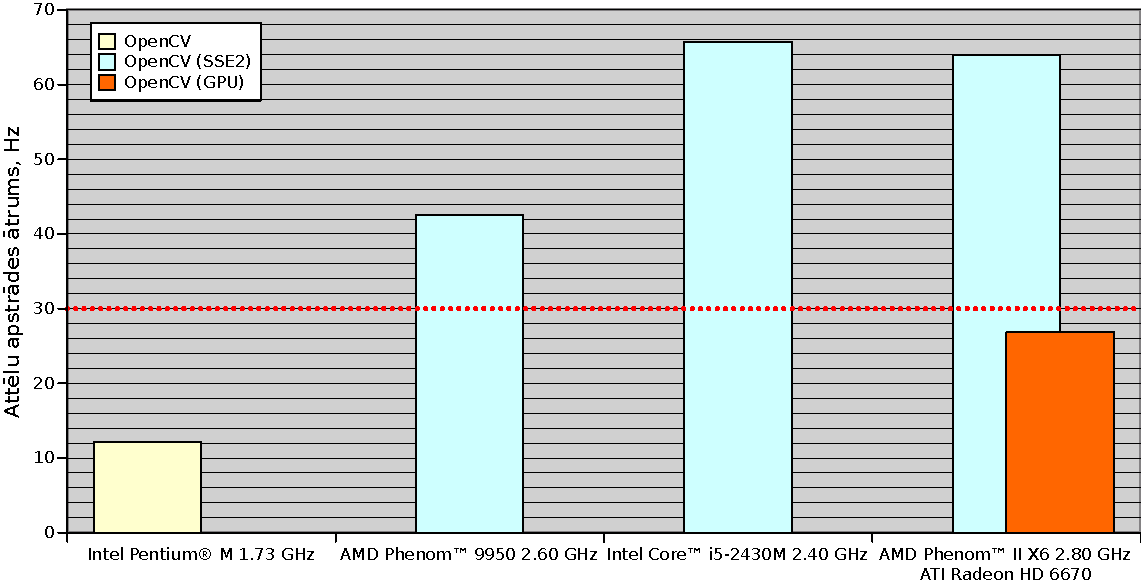
\includegraphics[width=0.9\linewidth]{chart-orb}
	\caption{Ātrdarbība OpenCV ORB implementāciju variantiem dažādās ierīcēs.}
	\label{fig:test4-data-text}
\end{figure}
Autors to skaidro ar nekorektu implementācijas modeli,
nevis platformas veiktspējas trūkumu.
Implementācijas \ref{tbl:orb-ocl-steps} tabulā uzskaitītie etapi,
ir atsevišķas OpenCL apakšprogrammas. Izsaucot OpenCL apakšprogrammu, datus
ir nepieciešams pārvietot uz GPU lokālo atmiņu (video atmiņu)~\cite{OpenCL-book}.
Ņemot vērā, ka katra no implementācijas apakšprogrammām izmanto attēla datus,
un vairums tiek izsauktas vairākkārtīgi, rezultātā vairums laika tiek patērēts
liekai datu pārraidei, šajā laikā skaitļošanas resursiem esot dīkstāvē.

Autora priekšlikums šīs problēmas risinājumam ir realizēt visu algoritmu
vienā OpenCL apakšprogrammā.




%~ \subsection{Potenciālās ātrdarbības uzlabojumu analīze}
%~ \TODO


}
	\caption{ORB algoritma blokshēma.}
	\label{fig:orb-sheem}
\end{figure}
Papildus lokālo maksimumu atlasei, ko veic FAST algoritms, ORB izmanto
Harisa (\termEn{Harris}) stūra mēru, lai no FAST raksturpunktiem atlasītu
$N$ skaitu labākos elementus~\cite{ORB}.
Rublē~u.c.\cite{ORB} to pamato ar relatīvi lielo FAST jutību attēla
objektu malām (pretstatā stūriem). Vienkāršota algoritma blokshēma attēlota
\ref{fig:orb-sheem}~attēlā.

FAST definīcija apskatīta \ref{sec:fast}~nodaļā
(\pageref{sec:fast}~lapā) un BRIEF definīcija --- \ref{sec:brief}~nodaļā
(\pageref{sec:brief}~lapā). Pārējās ORB algoritma komponenšu definīcijas
tiks apskatītas turpmākajās apakšnodaļās.

\subsection{Komponentes}
\subsubsection{Raksturpunktu atlase pēc Harisa mēra}
ORB izmanto FAST9 algoritma noteikto raksturpunktu pēcapstrādi novērtējot tos
pēc Harisa (\termEn{Harris}) stūru mēra un atlasot $N$ skaitu
raksturpunktus ar augstākajiem Harisa mēra rādītājiem~\cite{ORB}.
FAST detektora slieksnis $t$ tiek izvēlēts pietiekami zems, lai
raksturpunktu kopā būtu vismaz $N$ skaits elementu un $t$ tiek samazināts,
ja tā nav~\cite{ORB}.
Šī ir otrreizēja raksturpunktu atlase, jo tiek veikta pēc FAST 
lokālo maksimumu atlases.

%~ Harisa stūra mērs balstās uz starpību kvadrātu summu starp attēla
%~ apgabalu un no tā nobīdītiem apgabaliem, kura aprēķināšanai
%~ Haris\cite{Harris} definē aproksimācijas tenzoru~\cite{FAST}:
%~ \[
	%~ \vb{H} =
	%~ \begin{pmatrix}
		%~ \overline{{I_x'}^2} & \overline{{I_x'}{I_y'}}\\
		%~ \overline{{I_x'}{I_y'}} & \overline{{I_y'}^2}
	%~ \end{pmatrix}
%~ \]
%~ kur $I_x'$ un $I_y'$ ir attēla parciālie atvasinājumi (pēc $x$ un $y$),\\
%~ un
Harisa stūru mērs tiek izmantots Harisa stūru detektorā~\cite{Harris}\cite{FAST},
kuru aprēķina ar:
\begin{equation}
	V_H = |\vb{H}| - k \cdot {(H_{11}+H_{22})}^2
\end{equation}
kur\\
$\vb{H}$ ir Harisa matrica\cite{Harris}\cite{FAST}, un\\
%$H_{11}$ un $H_{22}$ ir $\vb{H}$ matricas elementi, un\\
$k$ ir konstante, kas kontrolē stūra vai malas jutību.

Harisa matrica $\vb{H}$, saīsinātā formā un izvērstā formā,
tiek pierakstīta kā~\cite{Harris}\cite{FAST}:
\begin{equation}\label{eq:harris}
	\vb{H} =
		\begin{pmatrix}
			\langle I_x^2 \rangle & \langle I_xI_y \rangle \\
			\langle I_xI_y \rangle & \langle I_y^2 \rangle
		\end{pmatrix}
		=
		\sum_{\vec{r}} W(\vec{r})
			\begin{pmatrix}
				I_x(\vec{p}+\vec{r})^2 & I_x(\vec{p}+\vec{r}) I_y(\vec{p}+\vec{r}) \\
				I_x(\vec{p}+\vec{r}) I_y(\vec{p}+\vec{r}) & I_y(\vec{p}+\vec{r})^2
			\end{pmatrix}
\end{equation}
kur\\
$I_x$ un $I_y$ ir parciālie atvasinājumi attēlam $\vb{I}$,\\
stūra iekavas $\langle {\,} \rangle$ apzīmē summēšanu noteiktā logā
(saīsinātā forma),\\
$W$ ir izvēlētais logs (kā funkcija), un\\
$\vec{r}$ ir loga pārvietojums no centra punkta $\vec{p}$, kurā tiek noteikta
intensitāšu starpība (atvasinājums).

%~ Harisa stūra detektors balstās uz noteikta attēla loga un tā pārvietojumu
%~ pašlīdzības noteikšanu ar starpību kvadrātu summu, ko
%~ aproksimē \eqref{eq:harris} definīcija~\cite{Harris}.

Hariss~un~Stefens\cite{Harris} (\termEn{Harris~and~Stephen})
rekomendē izmantot Gausa matricu par logu
$W$, bet avots~\cite{ORB}, definējot ORB, izmantotos parametrus nenorāda.
Autors analizējot ORB OpenCV implementācijas pirmkodu\cite{OpenCV-src}
secina, ka ORB implementācijā tiek izmantots $7 \times 7$ kvadrāta formas
logs (ar vienmērīgu sadalījumu) un izmantotais $k=0.04$.

Ņemot vērā, ka Harisa stūru mērs $V_H$ tiek noteikts punktiem
$\vec{p} \in \hat{F_9}(\vb{I}, \vec{p}, t)$, kas ir apakškopa no attēla
$\vb{I}$, pretstatā Harisa stūru detektoram, kas $V_H$ nosaka visiem attēla
punktiem~\cite{Harris}, var arī uzskatīt, ka šajā gadījumā FAST funkcionē kā
filtrs Harisa stūru detektoram.

\subsubsection{oFAST: raksturpunkta virziens} \label{sec:ofast}
oFAST ir ORB algoritma raksturpunktu virziena noteikšanas metode.
Neskatoties uz Rublē~u.c.\cite{ORB} piedēvēto nosaukumu, oFAST tiešā veidā
nemodificē FAST algoritmu un tādēļ autors to uzskata par atsevišķu ORB
algoritma komponenti.

Raksturpunktu virziena informācija ir nepieciešama
ORB rotācijas invariances nodrošināšanai~\cite{ORB}
(sk.~\ref{sec:rbrief-def}~nod.).
Tā noteikšanai izmanto
,,intensitātes centroīdu''\cite{Rosin}\cite{ORB} (jeb ,,masas'' centru, pēc fizikālās
līdzības), kas ir definēta kā:
\begin{equation}
	\vec{C} = \left( \frac{m_{10}}{m_{00}},\; \frac{m_{01}}{m_{00}} \right)
\end{equation}
kur $m_{00}$, $m_{01}$, $m_{10}$ ir attēla momenti, kurus aprēķina pēc:
\begin{equation}
	m_{pq} = \sum_{x,y} x^p y^p I(x,y)
\end{equation}

oFAST virzienu uzdod kā leņķi, kas vienāds ar centroīdas $\vec{C}$
lenķi pret $x$ asi (tās pozitīvo virzienu), ko aprēķina ar~\cite{ORB}:
\begin{equation}
	\theta = \mathrm{atan2}(m_{01}, m_{10})
\end{equation}
kur $\mathrm{atan2}()$ ir divu argumentu arktangenss (kas arī nosaka kvadrantu).

Lai šo virziena mēru padarītu maksimāli rotācijas invariantu,
momentu noteikšanai izvēlas riņķa formas attēla apgabalu ar diametru, kas
vienāds ar salāgotāja (kvadrāta formas) apgabala malas garumu $S$
(definēta~\ref{sec:brief}~nodaļā).

\subsubsection{rBRIEF deskriptors} \label{sec:rbrief-def}
rBRIEF ir rotācijas invarianta modifikācija
BRIEF deskriptoram (sk.~\ref{sec:brief}~nod.),
kura tiek izmantota par salāgošanas komponenti ORB
algoritmam. Idejas pamatā ir aprēķināt BRIEF deskriptoru izmantojot
rotētas salīdzināšanas pāru punktu koordinātes, rotācijas leņķi nosakot pēc
raksturpunkta virziena komponentes (sk.~\ref{sec:ofast}~nod.).

Apzīmēsim rBRIEF deskriptoru ar $D_{n_d}$, kuru mēs varam definēt
pievienojot BRIEF deskriptoram $B_{n_d}$ rotācijas komponenti ar leņķi $\theta$:
\begin{equation}\label{eq:rbrief}
	D_{n_d}(\hat{\vb{p}}, \theta) := \sum_{i=1}^{n_d} 2^{i-1}
		\tau\left(\hat{\vb{p}},
		          \vb{R}(\theta) \times \vb{a}_i,
		          \vb{R}(\theta) \times \vb{b}_i\right)
\end{equation}
kur $\vb{R}(\theta)$ ir rotācijas matrica leņķim $\theta$, kas ir definēta kā:
\[
	\vb{R}(\theta) = 
		\begin{pmatrix}
			\cos\theta & -\sin\theta\\
			\sin\theta & \cos\theta
		\end{pmatrix}
\]

Uzdotā definīcija \eqref{eq:rbrief} ir idejiski ekvivalenta bet 
pierakstīta ievērojami citādāk nekā \cite{ORB} avotā, jo 
Rublē~u.c. visai liberāli reinterpretē mainīgo nozīmi.

Jānorāda, ka nodrošinot rotācijas invarianci, šī informācija tiek
,,atmesta'' no deskriptora, kas samazina tā varianci un tādējādi arī
tā diskriminitāti. Rublē~u.c.\cite{ORB}, šī samazinājuma kompensēšanai,
izstrādā mašīnmācīšanās metodes, ar kuru palīdzību tiek izvēlēti
salīdzināšanas pāri ar augstāko varianci. Izvēlētie punkti attēloti
\ref{fig:pattern2}a.~attēlā un ir novērojama salīdzināšanu pāru tendence
orientēties raksturpunkta rotācijas virzienā (attēlā virzienā uz augšu).
\begin{figure}[tbh]
	\centering
	\def\svgwidth{0.7\linewidth}
	{\input{img/rBRIEF.pdf_tex}}
	\caption{Mašīnmācīšanās metožu izvēlēti salīdzināšanas pāri
		(attēloti 64 pāri)~\cite{ORB}.}
	\label{fig:pattern2}
\end{figure}
Bet ir arī novērojams, ka izvēlētie pāri ir izvietoti līdzīgi, kas palielina
to savstarpējo korelāciju
un tādējādi samazina to informatīvo vērtību. Rublē~u.c.\cite{ORB} izvēles
kritēriju papildina atlasot augstākās variances pārus, kuri atbilst
noteiktam korelācijas slieksnim (sk.~\ref{fig:pattern2}b.~att.), panākot
augstāku kopējo deskriptora diskriminitāti.



%~ \subsection{OpenCV ORB implementācija}
%~ \subsubsection{OpenCV ORB implementācija}
OpenCV biblotēka\cite{OpenCV-src} piedāvā ORB algoritma implementāciju.
Šī implementācija ir pielāgota secīgai izpildei CPU platformai,
bet tā ir pilnībā skalāra un nesatur būtiskus platformas specifiskus
ātrdarbības uzlabojumus (neskaitot \ref{sec:fast-ocv}~nod.~apskatīto
OpenCV FAST implementāciju, kas izmanto SSE2 SIMD instrukcijas).
rBRIEF salīdzināšanas pāri ir kodā definētas konstantes un
OpenCV nesatur ne saskarnes atbalstu, ne rīkus jaunas salīdzināšanas pāru 
kopas ģenerēšanai ar \ref{sec:rbrief-def}~nodaļā aprakstīto mašīnmācīšanās
metodi.

Rublē~u.c.\cite{ORB}, izstrādājot ORB, diskretizē virziena leņķi $\theta$ ar soli
$\frac{2\pi}{30}$ un aprēķina rBRIEF salīdzināšanas pāru koordinātas katrai no
$\theta$ ieņemamajām vērtībām, izveidojot apjomīgu
,,uzmeklēšanas datubāzi'' (\termEn{look-up table}).
OpenCV šo risinājumu nerealizē, tā vietā --- katra raksturpunkta
deskriptora
salīdzināšanas pāru punktu koordinātas tiek pārrēķinātas 
izmantojot rotācijas matricu kā definēts \eqref{eq:rbrief}~\cite{OpenCV-src}.

OpenCV ORB implementācija testos uzrādīja reāla laika spējīgu
apstrādes ātrumu --- virs 30 kadriem sekundē --- trim no četrām testētajām
ierīcēm (sk.~pielikumu~\ref{appx:test4}).
Salīdzinājums ar GPU implementāciju seko nākamajā (\ref{sec:orb-ocv-cl})
apakšnodaļā.

%~ \subsubsection{OpenCV ORB implementācijas OpenCL versija}
\subsubsection{OpenCL versija}
\label{sec:orb-ocv-cl}
OpenCV bibliotēka piedāvā arī OpenCL ORB versiju izpildei
GPU~\cite{OpenCV-src}. GPU implementācijas galvenā atšķirība no CPU versijas 
ir izpildes pavedienu izveide elementu apstrādei, bet, citādi,
algoritma implementācijas uzbūve ir identiska ar CPU implementāciju.
ORB algoritma OpenCL versijas izpildi var izdalīt vairākos etapos, kuri
uzskaitīti \ref{tbl:orb-ocl-steps}~tabulā.
\begin{table}[thb]\small
	\centering
	\caption{ORB GPU implementācijas izpildes etapi.}
	\label{tbl:orb-ocl-steps}
	\vspace{4pt}
	\begin{tabular}{clcl}
		\toprule
		\textbf{Nr.} & \textbf{Darbība} & $N_e$ & \textbf{Pavediena apstrādājamā vienība}\\
		\midrule
		1. & Attēlu piramīdas izveide & $N_L$ & Rezultējošā attēla pikselis\\
		2. & FAST9 punktu klasifikācija & $N_L$ & Attēla pikselis\\
		3. & FAST9 lokālo maksimumu atlase & $N_L$ & Raksturpunkts\\
		4. & Atlase pēc Harisa stūra mēra & 1 & Raksturpunkts\\
		5. & Intensitāšu centroīdu noteikšana & 1 & Raksturpunkts\\
		6. & Attēlu Gausa filtrēšana & $N_L$ & Rezultējošā attēla pikselis\\
		7. & rBRIEF deskriptoru aprēķins & 1 & Raksturpunkts\\
		\bottomrule
	\end{tabular}
	\begin{minipage}{0.6\linewidth}
		\noindent Apzīmējumi:\\
		$N_e$ --- etapa apakšprogrammas izsaukumu skaits\\
	\end{minipage}
\end{table}

Lai gan GPU teorētiskais skaitļošanas jaudas maksimums ir ievērojami lielāks
nekā CPU, šī ORB implementācija uzrādīja zemus ātrdarbības rādītājus testos
(sk.~\ref{fig:test4-data-text}~att.).
\begin{figure}[tbh]
	\centering
	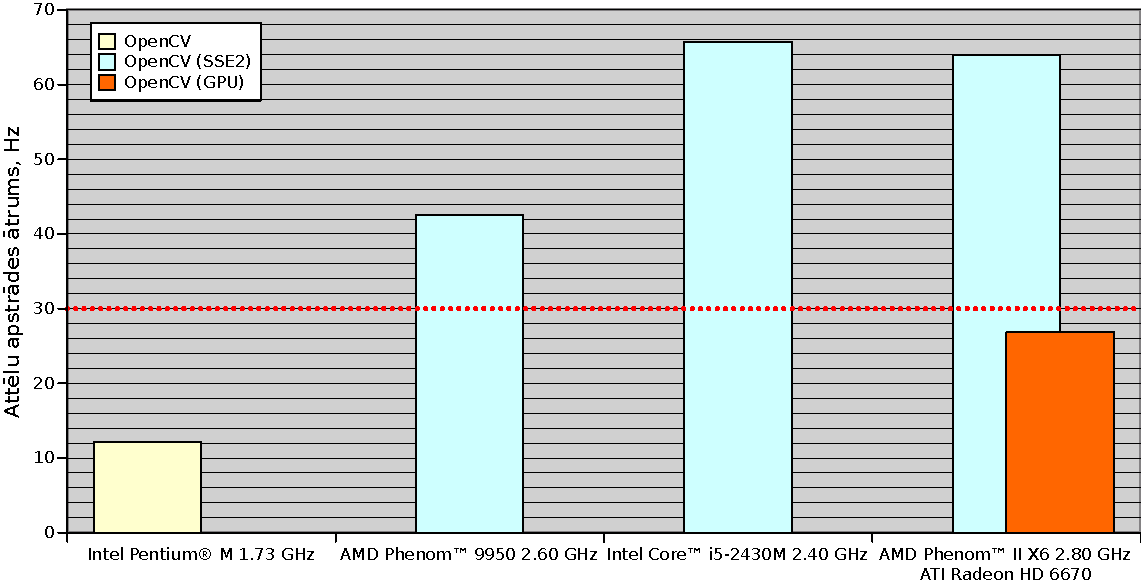
\includegraphics[width=0.9\linewidth]{chart-orb}
	\caption{Ātrdarbība OpenCV ORB implementāciju variantiem dažādās ierīcēs.}
	\label{fig:test4-data-text}
\end{figure}
Autors to skaidro ar nekorektu implementācijas modeli,
nevis platformas veiktspējas trūkumu.
Implementācijas \ref{tbl:orb-ocl-steps} tabulā uzskaitītie etapi,
ir atsevišķas OpenCL apakšprogrammas. Izsaucot OpenCL apakšprogrammu, datus
ir nepieciešams pārvietot uz GPU lokālo atmiņu (video atmiņu)~\cite{OpenCL-book}.
Ņemot vērā, ka katra no implementācijas apakšprogrammām izmanto attēla datus,
un vairums tiek izsauktas vairākkārtīgi, rezultātā vairums laika tiek patērēts
liekai datu pārraidei, šajā laikā skaitļošanas resursiem esot dīkstāvē.

Autora priekšlikums šīs problēmas risinājumam ir realizēt visu algoritmu
vienā OpenCL apakšprogrammā.




%~ \subsection{Potenciālās ātrdarbības uzlabojumu analīze}
%~ \TODO


}
	\caption{ORB algoritma blokshēma.}
	\label{fig:orb-sheem}
\end{figure}
Papildus lokālo maksimumu atlasei, ko veic FAST algoritms, ORB izmanto
Harisa (\termEn{Harris}) stūra mēru, lai no FAST raksturpunktiem atlasītu
$N$ skaitu labākos elementus~\cite{ORB}.
Rublē~u.c.\cite{ORB} to pamato ar relatīvi lielo FAST jutību attēla
objektu malām (pretstatā stūriem). Vienkāršota algoritma blokshēma attēlota
\ref{fig:orb-sheem}~attēlā.

FAST definīcija apskatīta \ref{sec:fast}~nodaļā
(\pageref{sec:fast}~lapā) un BRIEF definīcija --- \ref{sec:brief}~nodaļā
(\pageref{sec:brief}~lapā). Pārējās ORB algoritma komponenšu definīcijas
tiks apskatītas turpmākajās apakšnodaļās.

\subsection{Komponentes}
\subsubsection{Raksturpunktu atlase pēc Harisa mēra}
ORB izmanto FAST9 algoritma noteikto raksturpunktu pēcapstrādi novērtējot tos
pēc Harisa (\termEn{Harris}) stūru mēra un atlasot $N$ skaitu
raksturpunktus ar augstākajiem Harisa mēra rādītājiem~\cite{ORB}.
FAST detektora slieksnis $t$ tiek izvēlēts pietiekami zems, lai
raksturpunktu kopā būtu vismaz $N$ skaits elementu un $t$ tiek samazināts,
ja tā nav~\cite{ORB}.
Šī ir otrreizēja raksturpunktu atlase, jo tiek veikta pēc FAST 
lokālo maksimumu atlases.

%~ Harisa stūra mērs balstās uz starpību kvadrātu summu starp attēla
%~ apgabalu un no tā nobīdītiem apgabaliem, kura aprēķināšanai
%~ Haris\cite{Harris} definē aproksimācijas tenzoru~\cite{FAST}:
%~ \[
	%~ \vb{H} =
	%~ \begin{pmatrix}
		%~ \overline{{I_x'}^2} & \overline{{I_x'}{I_y'}}\\
		%~ \overline{{I_x'}{I_y'}} & \overline{{I_y'}^2}
	%~ \end{pmatrix}
%~ \]
%~ kur $I_x'$ un $I_y'$ ir attēla parciālie atvasinājumi (pēc $x$ un $y$),\\
%~ un
Harisa stūru mērs tiek izmantots Harisa stūru detektorā~\cite{Harris}\cite{FAST},
kuru aprēķina ar:
\begin{equation}
	V_H = |\vb{H}| - k \cdot {(H_{11}+H_{22})}^2
\end{equation}
kur\\
$\vb{H}$ ir Harisa matrica\cite{Harris}\cite{FAST}, un\\
%$H_{11}$ un $H_{22}$ ir $\vb{H}$ matricas elementi, un\\
$k$ ir konstante, kas kontrolē stūra vai malas jutību.

Harisa matrica $\vb{H}$, saīsinātā formā un izvērstā formā,
tiek pierakstīta kā~\cite{Harris}\cite{FAST}:
\begin{equation}\label{eq:harris}
	\vb{H} =
		\begin{pmatrix}
			\langle I_x^2 \rangle & \langle I_xI_y \rangle \\
			\langle I_xI_y \rangle & \langle I_y^2 \rangle
		\end{pmatrix}
		=
		\sum_{\vec{r}} W(\vec{r})
			\begin{pmatrix}
				I_x(\vec{p}+\vec{r})^2 & I_x(\vec{p}+\vec{r}) I_y(\vec{p}+\vec{r}) \\
				I_x(\vec{p}+\vec{r}) I_y(\vec{p}+\vec{r}) & I_y(\vec{p}+\vec{r})^2
			\end{pmatrix}
\end{equation}
kur\\
$I_x$ un $I_y$ ir parciālie atvasinājumi attēlam $\vb{I}$,\\
stūra iekavas $\langle {\,} \rangle$ apzīmē summēšanu noteiktā logā
(saīsinātā forma),\\
$W$ ir izvēlētais logs (kā funkcija), un\\
$\vec{r}$ ir loga pārvietojums no centra punkta $\vec{p}$, kurā tiek noteikta
intensitāšu starpība (atvasinājums).

%~ Harisa stūra detektors balstās uz noteikta attēla loga un tā pārvietojumu
%~ pašlīdzības noteikšanu ar starpību kvadrātu summu, ko
%~ aproksimē \eqref{eq:harris} definīcija~\cite{Harris}.

Hariss~un~Stefens\cite{Harris} (\termEn{Harris~and~Stephen})
rekomendē izmantot Gausa matricu par logu
$W$, bet avots~\cite{ORB}, definējot ORB, izmantotos parametrus nenorāda.
Autors analizējot ORB OpenCV implementācijas pirmkodu\cite{OpenCV-src}
secina, ka ORB implementācijā tiek izmantots $7 \times 7$ kvadrāta formas
logs (ar vienmērīgu sadalījumu) un izmantotais $k=0.04$.

Ņemot vērā, ka Harisa stūru mērs $V_H$ tiek noteikts punktiem
$\vec{p} \in \hat{F_9}(\vb{I}, \vec{p}, t)$, kas ir apakškopa no attēla
$\vb{I}$, pretstatā Harisa stūru detektoram, kas $V_H$ nosaka visiem attēla
punktiem~\cite{Harris}, var arī uzskatīt, ka šajā gadījumā FAST funkcionē kā
filtrs Harisa stūru detektoram.

\subsubsection{oFAST: raksturpunkta virziens} \label{sec:ofast}
oFAST ir ORB algoritma raksturpunktu virziena noteikšanas metode.
Neskatoties uz Rublē~u.c.\cite{ORB} piedēvēto nosaukumu, oFAST tiešā veidā
nemodificē FAST algoritmu un tādēļ autors to uzskata par atsevišķu ORB
algoritma komponenti.

Raksturpunktu virziena informācija ir nepieciešama
ORB rotācijas invariances nodrošināšanai~\cite{ORB}
(sk.~\ref{sec:rbrief-def}~nod.).
Tā noteikšanai izmanto
,,intensitātes centroīdu''\cite{Rosin}\cite{ORB} (jeb ,,masas'' centru, pēc fizikālās
līdzības), kas ir definēta kā:
\begin{equation}
	\vec{C} = \left( \frac{m_{10}}{m_{00}},\; \frac{m_{01}}{m_{00}} \right)
\end{equation}
kur $m_{00}$, $m_{01}$, $m_{10}$ ir attēla momenti, kurus aprēķina pēc:
\begin{equation}
	m_{pq} = \sum_{x,y} x^p y^p I(x,y)
\end{equation}

oFAST virzienu uzdod kā leņķi, kas vienāds ar centroīdas $\vec{C}$
lenķi pret $x$ asi (tās pozitīvo virzienu), ko aprēķina ar~\cite{ORB}:
\begin{equation}
	\theta = \mathrm{atan2}(m_{01}, m_{10})
\end{equation}
kur $\mathrm{atan2}()$ ir divu argumentu arktangenss (kas arī nosaka kvadrantu).

Lai šo virziena mēru padarītu maksimāli rotācijas invariantu,
momentu noteikšanai izvēlas riņķa formas attēla apgabalu ar diametru, kas
vienāds ar salāgotāja (kvadrāta formas) apgabala malas garumu $S$
(definēta~\ref{sec:brief}~nodaļā).

\subsubsection{rBRIEF deskriptors} \label{sec:rbrief-def}
rBRIEF ir rotācijas invarianta modifikācija
BRIEF deskriptoram (sk.~\ref{sec:brief}~nod.),
kura tiek izmantota par salāgošanas komponenti ORB
algoritmam. Idejas pamatā ir aprēķināt BRIEF deskriptoru izmantojot
rotētas salīdzināšanas pāru punktu koordinātes, rotācijas leņķi nosakot pēc
raksturpunkta virziena komponentes (sk.~\ref{sec:ofast}~nod.).

Apzīmēsim rBRIEF deskriptoru ar $D_{n_d}$, kuru mēs varam definēt
pievienojot BRIEF deskriptoram $B_{n_d}$ rotācijas komponenti ar leņķi $\theta$:
\begin{equation}\label{eq:rbrief}
	D_{n_d}(\hat{\vb{p}}, \theta) := \sum_{i=1}^{n_d} 2^{i-1}
		\tau\left(\hat{\vb{p}},
		          \vb{R}(\theta) \times \vb{a}_i,
		          \vb{R}(\theta) \times \vb{b}_i\right)
\end{equation}
kur $\vb{R}(\theta)$ ir rotācijas matrica leņķim $\theta$, kas ir definēta kā:
\[
	\vb{R}(\theta) = 
		\begin{pmatrix}
			\cos\theta & -\sin\theta\\
			\sin\theta & \cos\theta
		\end{pmatrix}
\]

Uzdotā definīcija \eqref{eq:rbrief} ir idejiski ekvivalenta bet 
pierakstīta ievērojami citādāk nekā \cite{ORB} avotā, jo 
Rublē~u.c. visai liberāli reinterpretē mainīgo nozīmi.

Jānorāda, ka nodrošinot rotācijas invarianci, šī informācija tiek
,,atmesta'' no deskriptora, kas samazina tā varianci un tādējādi arī
tā diskriminitāti. Rublē~u.c.\cite{ORB}, šī samazinājuma kompensēšanai,
izstrādā mašīnmācīšanās metodes, ar kuru palīdzību tiek izvēlēti
salīdzināšanas pāri ar augstāko varianci. Izvēlētie punkti attēloti
\ref{fig:pattern2}a.~attēlā un ir novērojama salīdzināšanu pāru tendence
orientēties raksturpunkta rotācijas virzienā (attēlā virzienā uz augšu).
\begin{figure}[tbh]
	\centering
	\def\svgwidth{0.7\linewidth}
	{\input{img/rBRIEF.pdf_tex}}
	\caption{Mašīnmācīšanās metožu izvēlēti salīdzināšanas pāri
		(attēloti 64 pāri)~\cite{ORB}.}
	\label{fig:pattern2}
\end{figure}
Bet ir arī novērojams, ka izvēlētie pāri ir izvietoti līdzīgi, kas palielina
to savstarpējo korelāciju
un tādējādi samazina to informatīvo vērtību. Rublē~u.c.\cite{ORB} izvēles
kritēriju papildina atlasot augstākās variances pārus, kuri atbilst
noteiktam korelācijas slieksnim (sk.~\ref{fig:pattern2}b.~att.), panākot
augstāku kopējo deskriptora diskriminitāti.



%~ \subsection{OpenCV ORB implementācija}
%~ \subsubsection{OpenCV ORB implementācija}
OpenCV biblotēka\cite{OpenCV-src} piedāvā ORB algoritma implementāciju.
Šī implementācija ir pielāgota secīgai izpildei CPU platformai,
bet tā ir pilnībā skalāra un nesatur būtiskus platformas specifiskus
ātrdarbības uzlabojumus (neskaitot \ref{sec:fast-ocv}~nod.~apskatīto
OpenCV FAST implementāciju, kas izmanto SSE2 SIMD instrukcijas).
rBRIEF salīdzināšanas pāri ir kodā definētas konstantes un
OpenCV nesatur ne saskarnes atbalstu, ne rīkus jaunas salīdzināšanas pāru 
kopas ģenerēšanai ar \ref{sec:rbrief-def}~nodaļā aprakstīto mašīnmācīšanās
metodi.

Rublē~u.c.\cite{ORB}, izstrādājot ORB, diskretizē virziena leņķi $\theta$ ar soli
$\frac{2\pi}{30}$ un aprēķina rBRIEF salīdzināšanas pāru koordinātas katrai no
$\theta$ ieņemamajām vērtībām, izveidojot apjomīgu
,,uzmeklēšanas datubāzi'' (\termEn{look-up table}).
OpenCV šo risinājumu nerealizē, tā vietā --- katra raksturpunkta
deskriptora
salīdzināšanas pāru punktu koordinātas tiek pārrēķinātas 
izmantojot rotācijas matricu kā definēts \eqref{eq:rbrief}~\cite{OpenCV-src}.

OpenCV ORB implementācija testos uzrādīja reāla laika spējīgu
apstrādes ātrumu --- virs 30 kadriem sekundē --- trim no četrām testētajām
ierīcēm (sk.~pielikumu~\ref{appx:test4}).
Salīdzinājums ar GPU implementāciju seko nākamajā (\ref{sec:orb-ocv-cl})
apakšnodaļā.

%~ \subsubsection{OpenCV ORB implementācijas OpenCL versija}
\subsubsection{OpenCL versija}
\label{sec:orb-ocv-cl}
OpenCV bibliotēka piedāvā arī OpenCL ORB versiju izpildei
GPU~\cite{OpenCV-src}. GPU implementācijas galvenā atšķirība no CPU versijas 
ir izpildes pavedienu izveide elementu apstrādei, bet, citādi,
algoritma implementācijas uzbūve ir identiska ar CPU implementāciju.
ORB algoritma OpenCL versijas izpildi var izdalīt vairākos etapos, kuri
uzskaitīti \ref{tbl:orb-ocl-steps}~tabulā.
\begin{table}[thb]\small
	\centering
	\caption{ORB GPU implementācijas izpildes etapi.}
	\label{tbl:orb-ocl-steps}
	\vspace{4pt}
	\begin{tabular}{clcl}
		\toprule
		\textbf{Nr.} & \textbf{Darbība} & $N_e$ & \textbf{Pavediena apstrādājamā vienība}\\
		\midrule
		1. & Attēlu piramīdas izveide & $N_L$ & Rezultējošā attēla pikselis\\
		2. & FAST9 punktu klasifikācija & $N_L$ & Attēla pikselis\\
		3. & FAST9 lokālo maksimumu atlase & $N_L$ & Raksturpunkts\\
		4. & Atlase pēc Harisa stūra mēra & 1 & Raksturpunkts\\
		5. & Intensitāšu centroīdu noteikšana & 1 & Raksturpunkts\\
		6. & Attēlu Gausa filtrēšana & $N_L$ & Rezultējošā attēla pikselis\\
		7. & rBRIEF deskriptoru aprēķins & 1 & Raksturpunkts\\
		\bottomrule
	\end{tabular}
	\begin{minipage}{0.6\linewidth}
		\noindent Apzīmējumi:\\
		$N_e$ --- etapa apakšprogrammas izsaukumu skaits\\
	\end{minipage}
\end{table}

Lai gan GPU teorētiskais skaitļošanas jaudas maksimums ir ievērojami lielāks
nekā CPU, šī ORB implementācija uzrādīja zemus ātrdarbības rādītājus testos
(sk.~\ref{fig:test4-data-text}~att.).
\begin{figure}[tbh]
	\centering
	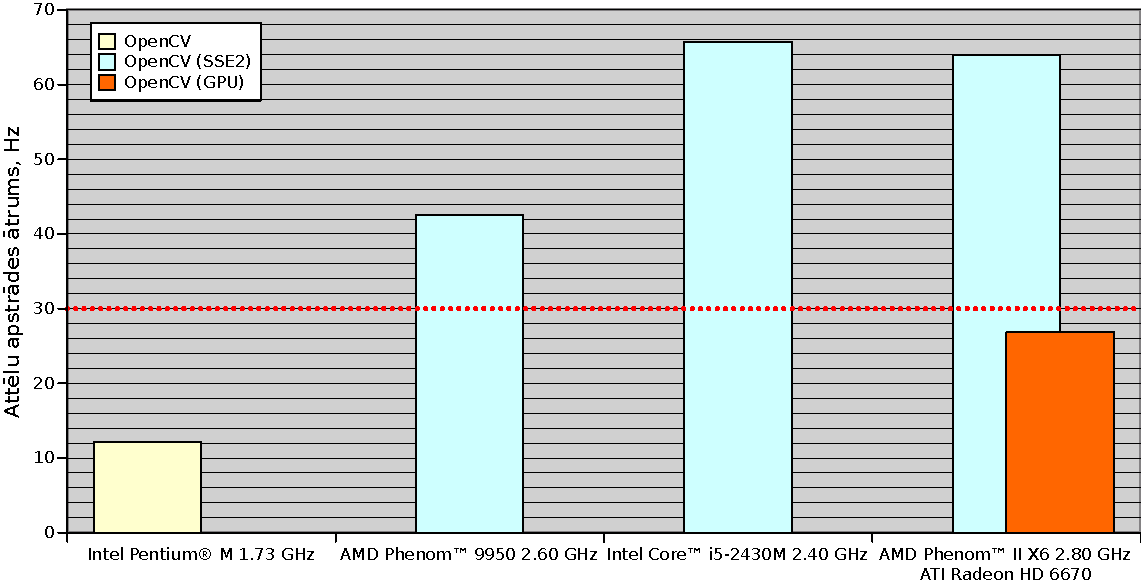
\includegraphics[width=0.9\linewidth]{chart-orb}
	\caption{Ātrdarbība OpenCV ORB implementāciju variantiem dažādās ierīcēs.}
	\label{fig:test4-data-text}
\end{figure}
Autors to skaidro ar nekorektu implementācijas modeli,
nevis platformas veiktspējas trūkumu.
Implementācijas \ref{tbl:orb-ocl-steps} tabulā uzskaitītie etapi,
ir atsevišķas OpenCL apakšprogrammas. Izsaucot OpenCL apakšprogrammu, datus
ir nepieciešams pārvietot uz GPU lokālo atmiņu (video atmiņu)~\cite{OpenCL-book}.
Ņemot vērā, ka katra no implementācijas apakšprogrammām izmanto attēla datus,
un vairums tiek izsauktas vairākkārtīgi, rezultātā vairums laika tiek patērēts
liekai datu pārraidei, šajā laikā skaitļošanas resursiem esot dīkstāvē.

Autora priekšlikums šīs problēmas risinājumam ir realizēt visu algoritmu
vienā OpenCL apakšprogrammā.




%~ \subsection{Potenciālās ātrdarbības uzlabojumu analīze}
%~ \TODO


